\section{Máquinas de estados finitos}

Con máquinas de estados finitos se modelaron clientes compitiendo por recursos
limitados --- en este caso unidades --- en el contexto de \textit{una} compra.
Por lo tanto \texttt{carrito confirmado} es un estado terminal.
No se modeló la posibilidad de hacer nuevas compras ya que eso requeriría
terminar la compra actual y por lo tanto modelar todo el comportamiento de
depósito y logística, aspectos que consideramos ya están bien enunciados con
otros modelos.

\begin{figure}[H]
  \begin{center}
  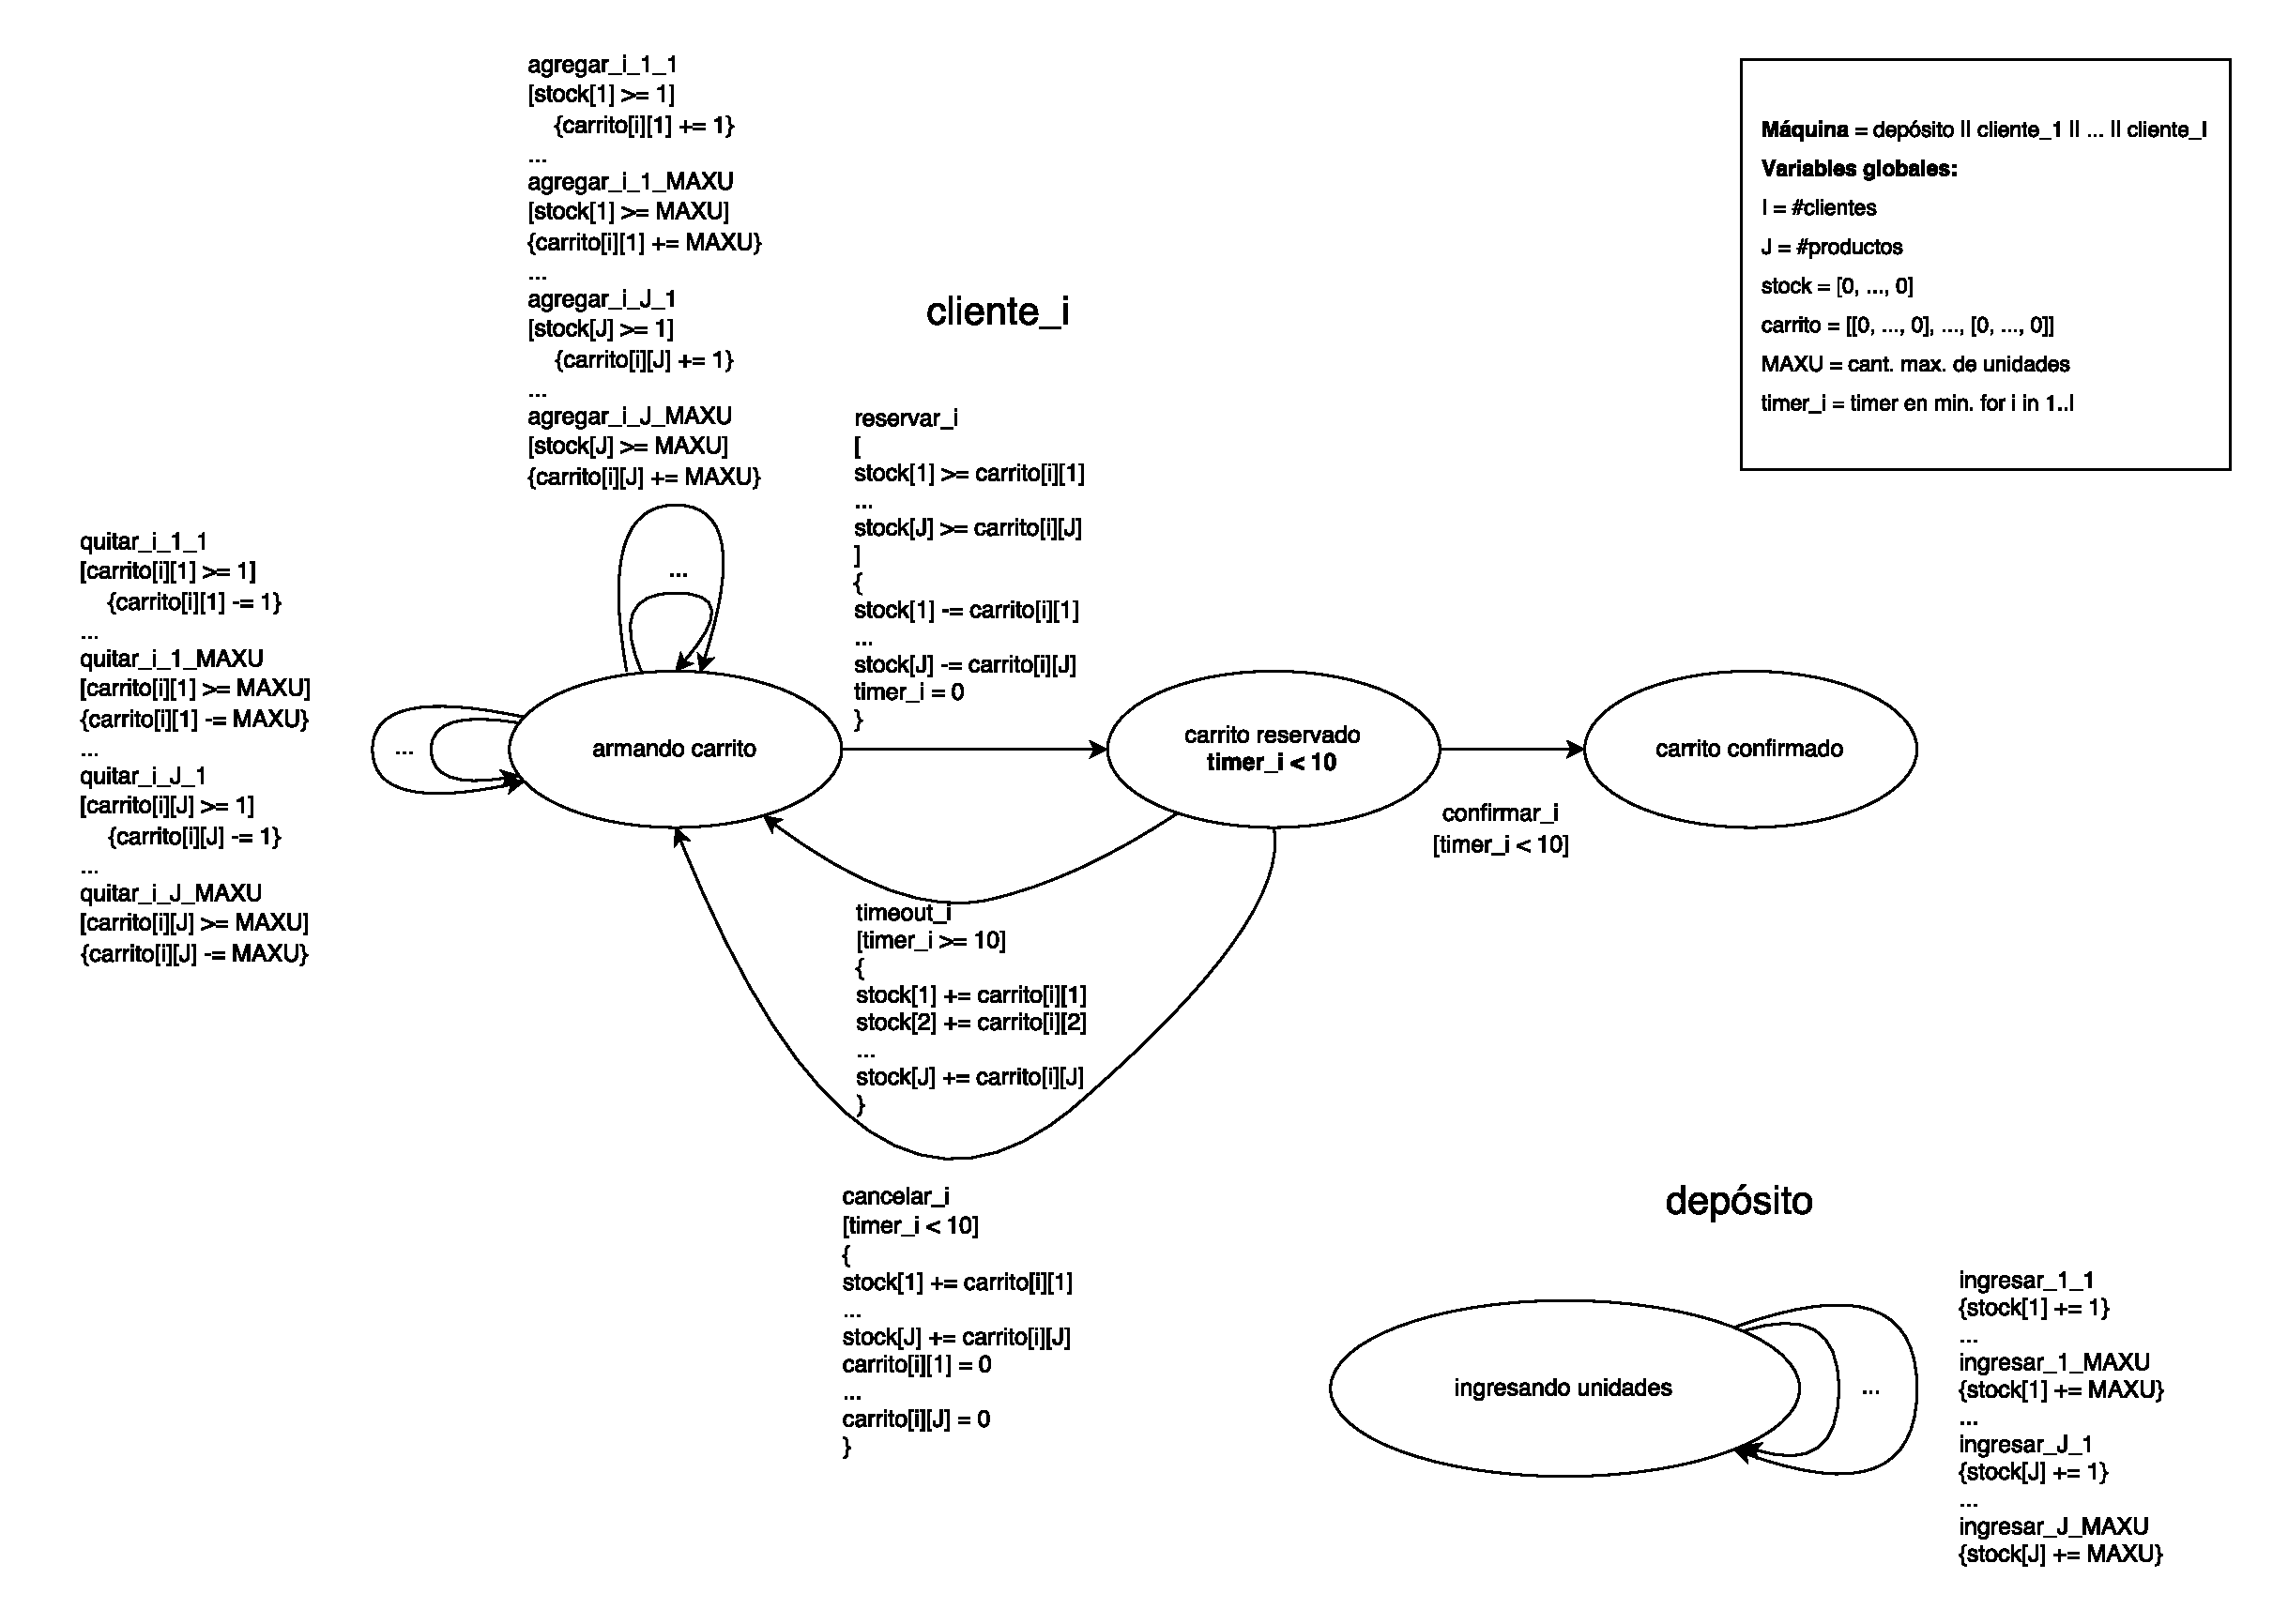
\includegraphics[angle=90,height=\textheight]{tp2/images/fsm.pdf}
  \end{center}
\end{figure}
